%************************************************
\chapter{Resultados}\label{ch:resultados}
%************************************************

Este capítulo muestra los resultados de la estimación de parámetros para la construcción de modelos de ecuaciones de Glass tanto para la red de tres nodos del apéndice \ref{ch:3Nodos} como para la vía de señalización de speract presentada en el capítulo \ref{ch:antecedentes}. Posteriormente se presenta una breve discusión de los resultados.


\section{Modelo de tres nodos}

Como caso de ejemplo de estimación de parámetros en un problema de transformación de un modelo discreto a un modelo semicontinuo, se resolvió mediante el método de Euler el sistema de ecuaciones de Glass de la red de 3 nodos con parámetros $\alpha_{\sigma_x} = \alpha_{\sigma_y} =  \alpha_{\sigma_z} = 1$, umbrales de activación $\theta_{\sigma_x} = 0.3$, $\theta_{\sigma_y} = 0.7$ y $\theta_{\sigma_z} = 0.8$, y $\sigma_x = 1$, $\sigma_y = 0$, $\sigma_z = 0$ como condiciones iniciales. El objetivo consistió en encontrar mediante un procedimiento de búsqueda el conjunto de parámetros tales que la dinámica de Glass correspondiente al $\sigma_x$ fuera lo más similar posible a la solución conocida para los parámetros antes mencionados. Esta solución conocida se tomó como una señal artificial, que se muestra en la figura \ref{fig:signal3nodos}.

\begin{figure}[hbt]
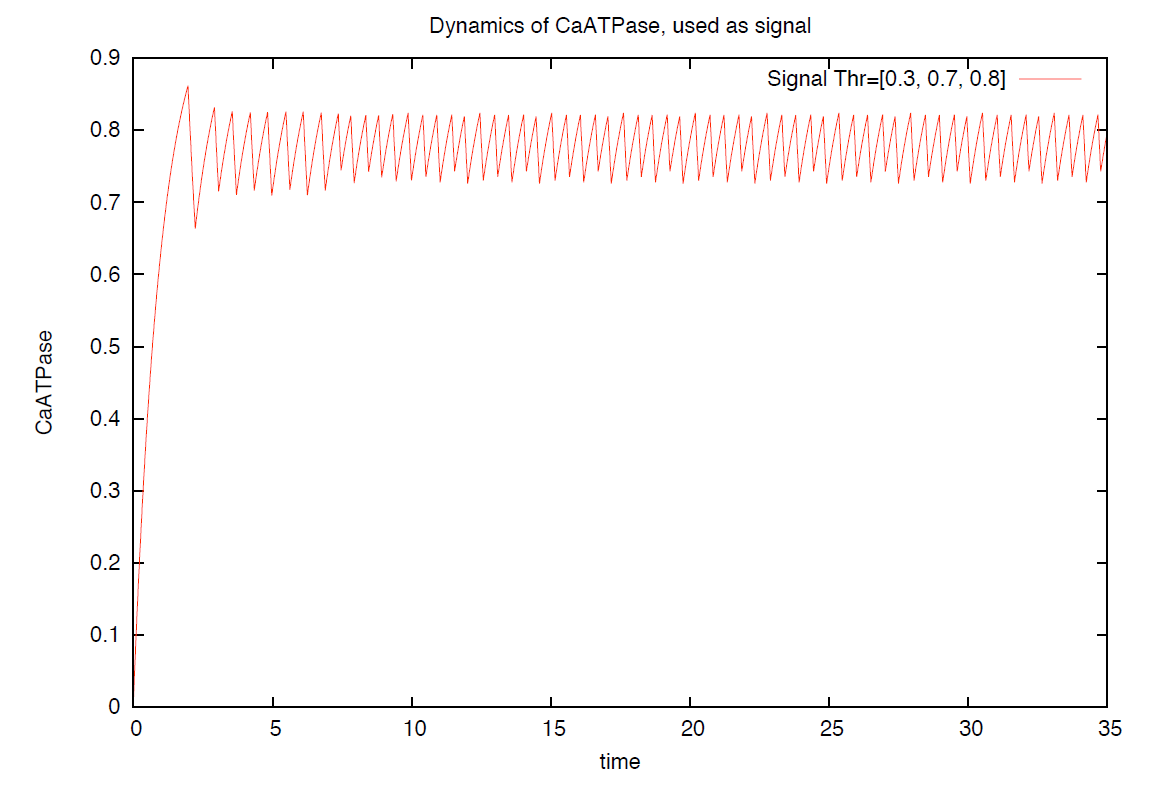
\includegraphics[width=0.9\linewidth]{gfx/original3Nodos}
\caption[Dinámica original $\sigma_z$]{Solución del problema de condiciones iniciales $\sigma_x = 1$, $\sigma_y = 0$, $\sigma_z = 0$ de las ecuaciones \ref{glass1_3nodos}, \ref{glass2_3nodos} y \ref{glass3_3nodos}, correspondientes al modelo de Glass de la red de 3 nodos del apéndice \ref{ch:3Nodos}, con parámetros $\alpha_{\sigma_x} = \alpha_{\sigma_y} = \alpha_{\sigma_z} = 1$, umbrales de activación $\theta_{\sigma_x} = 0.3$, $\theta_{\sigma_y} = 0.7$ y $\theta_{\sigma_z} = 0.8$. Se muestra la solución con respecto a tiempo de $\sigma_z$.}\label{fig:signal3nodos}
\end{figure}

Se eligió búsqueda aleatoria como estrategia de exploración del espacio de búsqueda, mientras que la función objetivo consistió en minimizar $f_{SI}(X,Y) = 1 -SI(X,Y)$ con $X$ la señal original y $Y$ los datos de la dinámica de Glass del nodo $\sigma_z$ de cada uno de los candidatos propuestos por el algoritmo de búsqueda.

\begin{figure}[hbt]
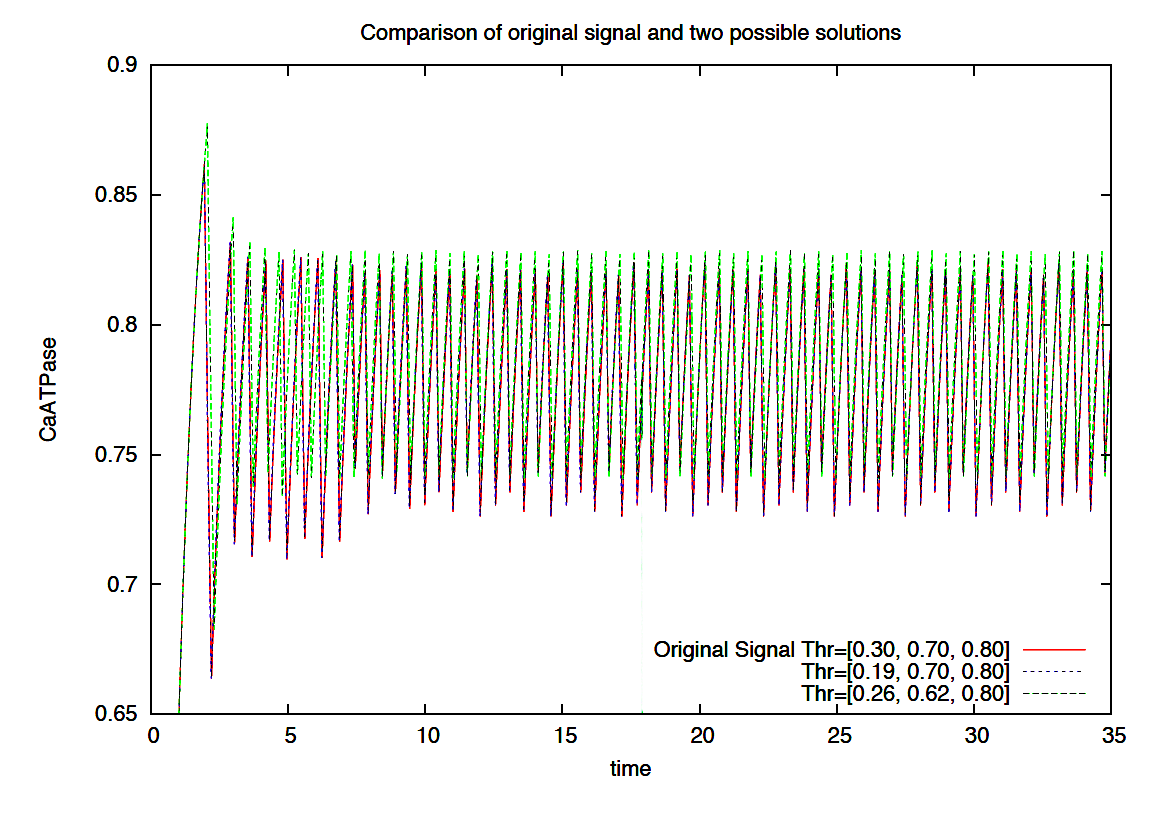
\includegraphics[width=0.9\linewidth]{gfx/comparacion3Nodos}
\caption[Dinámicas original y estimada $\sigma_z$]{Dinámicas original y estimada de $\sigma_z$ de la red de 3 nodos. En rojo la señal original, verde y azul representan dos distintas ejecuciones del programa de búsqueda.}\label{fig:resultadoChido3Nodos}
\end{figure}

En este caso, fue posible recuperar el valor de los tres parámetros de umbral $\theta_{\sigma_x}, \theta_{\sigma_y}, \theta_{\sigma_z}$ en varias ejecuciones del programa de búsqueda. La figura \ref{fig:resultadoChido3Nodos} muestra la dinámica original y el resultado obtenido con dos ejecuciones distintas del programa de busqueda.

Se probó realizar la estimación de parámetros para el mismo sistema usando una versión de algoritmos genéticos adaptada a problemas con variables continuas con los parámetros recomendados por omision, tal como se refiere en \citeauthor{Haupt1998} \citep{Haupt1998}. En este caso fue posible recuperar el valor del parámetro de umbral para $\sigma_z$, si bien con una precisión menor.
% Después tal vez sea bueno agregar los resultados a un apéndice.

Cabe mencionar que a pesar de que este caso de ejemplo no está relacionado en un sentido bioquímico con la red de señalización de speract, sí lo está en términos de ser un modelo discreto que se quiere reescribir como semicontinuo. Además, para la estimación de parámetros se usó un solo tipo de señal o ``medición experimental'' contra la cual comparar la dinámica de cada uno de los candidatos, situación que se presentó también en la red de señalización, donde solo se cuenta con un único tipo de mediciones para tiempos largos. La experiencia ganada con este caso de ejemplo sirvió como base para abordar la estimación de parámetros del modelo semicontinuo de la vía de señalización de speract.

\section{Modelo de la red de señalización}

El modelo semicontinuo de la vía de señalización de speract se implementó planteando ecuaciones de Glass cuyo valor depende de un conjunto de funciones discretas, estas últimas basadas en el modelo de \citeauthor{Espinal2011} \citep{Espinal2011}.%La implementación en lenguaje C de dichas funciones discretas se muestran en el apéndice \ref{ch:appendix}.
A modo de ejemplo, puede considerarse la ecuación de Glass para \acf{gc}. La función Booleana para este nodo de la red es

\begin{eqnarray}
\ac{gc} & = & F_{\ac{gc}} \left( \ac{SR} \wedge \neg \ac{phi} \right)
\end{eqnarray}
\\
y la ecuación de Glass correspondiente es

\begin{eqnarray}\label{eqn:glasscGMP}
\frac{d\ac{gc}}{dt} & = & \alpha_{\ac{gc}} [F_{\ac{gc}}(\widehat{\ac{SR}}, \widehat{\ac{phi}}) - \ac{gc}]
\end{eqnarray}
\\
donde
\begin{eqnarray}
\widehat{\ac{SR}} & = & H(\ac{SR} - \theta_{\ac{SR}})\\
\widehat{\ac{phi}} & = & H(\ac{phi} - \theta_{\ac{phi}})
\end{eqnarray}
\\
son los valores discretizados de las variables continuas \acf{SR} y \acf{phi}, respectivamente.

El problema de estimación de parámetros en este caso consiste en ajustar el valor de 26 parámetros de umbral $\theta_i$ (22 para los nodos binarios y 4 extras para los nodos que tienen un valor terciario), en el caso de un sistema sincronizado donde todos los parámetros $\alpha_i=x$, $x \in [0,T_{max}]$, donde $T_{max}$ es el tiempo característico más grande del sistema. 

Un problema similar, si bien más complicado, es permitir que cada $\alpha_i$ tome un valor distinto de los demás $\alpha_i$, es decir, un problema asíncrono. El problema asíncrono añade la necesidad de estimar 22 parámetros extra, uno para cada componente del sistema.

Como una primera aproximación al problema, se consideró el problema sincronizado, estableciendo $\alpha_i = 1.0\ \forall i$, de modo que solo se debió estimar el valor de los 26 parámetros de umbral. Las condiciones iniciales se fijaron tales que al discretizar los valores continuos de la condición inicial, se tuviera una situación muy similar a la del organismo silvestre o \emph{wild type}, es decir, aquél al que no se le ha hecho modificación alguna. Tras la discretización de los valores continuos, la condición inicial del modelo semicontinuo es similar a la condición inicial del modelo discreto presentado en la sección \ref{sect:erizo}, tal y como fue presentada en la figura \ref{fig:appletErizo}.

En particular la condición inicial del modelo de ecuaciones de Glass para la vía de señalización se estableció con los valores
\begin{eqnarray*}
\ac{v} & = & 1.0\\
\ac{hva} & = & 1.0\\
\ac{lva} & = & 1.0\\
\ac{calintra} & = & 0.9\\
\text{Todos los demás } & = & 0.2 
\end{eqnarray*}
\\
Estos valores indican, como se mencionó en el pie de la figura \ref{fig:appletErizo} de la sección \ref{sect:erizo}, estados en los que el \acf{v} está en el estado que representa la hiperpolarización de la membrana del flagelo, los canales \acf{hva} y \acf{lva} se encuentran activos (pero no abiertos) y el \acf{calintra} está en un valor muy cercano al inicio de las oscilaciones tónicas.

En vista de que aun para el problema sincronizado el espacio de parámetros es mayor que el del problema de 3 nodos presentado en la sección anterior, y de que los algoritmos genéticos no presentaron una mejora con respecto a la búsqueda aleatoria en el mismo problema, se buscó otro método de exploración del espacio de búsqueda. A este respecto, \citeauthor{BangaMoles2003} \citep{BangaMoles2003} muestran que para problemas de estimación de parámetros en redes de señalización bioquímica los métodos con mejores resultados son aquellos basados en estrategias evolutivas. En especial algunos como Evolución Diferencial resultan aún mejores que los algoritmos genéticos.

Para la búsqueda de parámetros de la vía de señalización de speract se usó entonces Evolución Diferencial como estrategia de búsqueda (y evaluación de candidatos), usando los parámetros recomendados en la literatura \citeauthor{Storn1997}  \citep{Storn1997}. Para comparar la dinámica del nodo de $Ca^{2+}$, (denotado en el modelo como $dCa$) de cada modelo planteado con las mediciones experimentales de fluorescencia de $Ca^{2+}$, se buscó minimizar $f_{Pearson}(X,Y) = 1-r_{X,Y}$, donde $X$ son los datos experimentales y $Y$ son los datos de la dinámica del nodo de calcio del modelo. 

Los sistemas de ecuaciones de Glass se resolvieron mediante el método solución de ecuaciones diferenciales de Euler. Para algunas dinámicas elegidas por el algoritmo de Evolución Diferencial presentado en \ref{difEvol}, se verificó la solución usando el método para solución de ecuaciones diferenciales ordinarias de Adams-Bashforth, \citeauthor{gslManual} \citep{gslManual}. No se encontraron diferencias significativas entre las soluciones de uno y otro métodos.

Se logró ajustar la dinámica del nodo de $Ca^{2+}$ de acuerdo a mediciones experimentales, como se muestra en la figura \ref{fig:glassChido}. 

\begin{figure}[h]
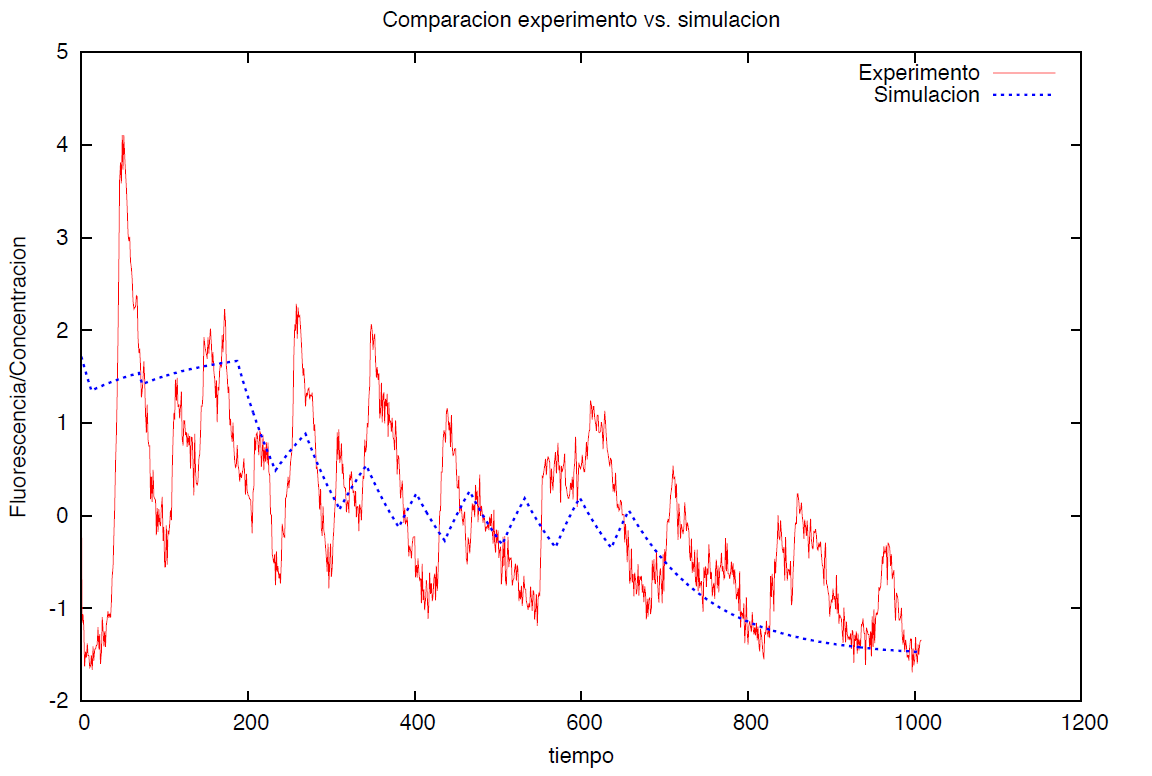
\includegraphics[width=0.9\linewidth]{gfx/glassChido}
\caption[Dinámica del nodo de $Ca^{2+}$ del modelo y medición experimental de $Ca^{2+}$]{Dinámica del nodo de $Ca^{2+}$ del modelo y medición experimental de $Ca^{2+}$. En rojo la medición experimental, en azul el ajuste usando la función objetivo basada en la correlación de Pearson. Para efectos de comparación, las series se normalizaron de manera que tuvieran promedio $0$ y varianza $1$.}\label{fig:glassChido}
\end{figure}

A pesar de lo alentador de este resultado, el comportamiento dinámico de otros nodos aún necesita mayor revisión. Por ejemplo, el nodo correspondiente al potencial de membrana $V$ debería de disminuir su valor al inicio de la dinámica para luego aumentarlo. Sin embargo, el potencial aumenta al principio y disminuye posteriormente. Este comportamiento es imposible en la realidad, ya que al haber un aumento de $[Ca^{2+}]_i$ el potencial deberia disminuir. Véase la figura \ref{fig:glassChafa}.

\begin{figure}[h]
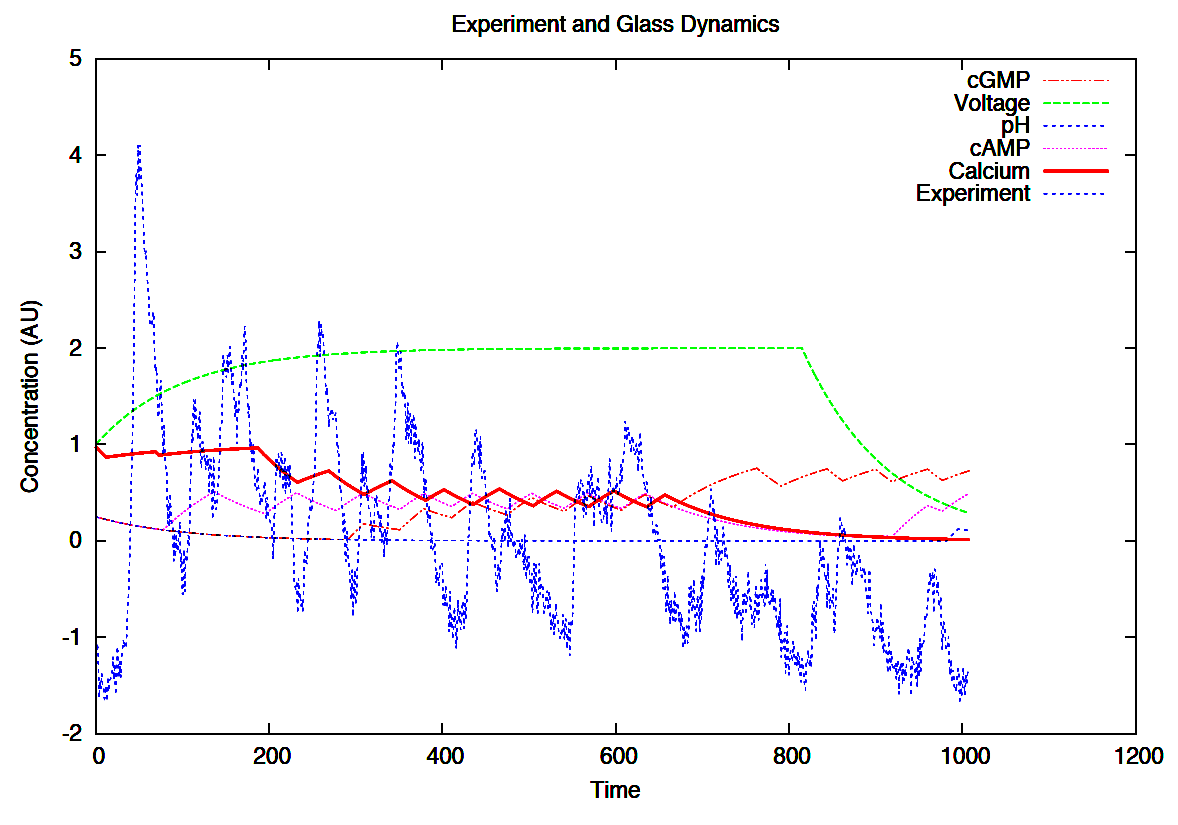
\includegraphics[width=0.9\linewidth]{gfx/glassChafa}
\caption[Dinámica de $Ca^{2+}$, $V$ y otros componentes del modelo, y medición experimental de $Ca^{2+}$]{Dinámica del nodo de $Ca^{2+}$, $V$ y otros componentes del modelo, y medición experimental de $Ca^{2+}$. En este caso en azul punteado se muestra la medición expetimental, en rojo el nodo de $Ca^{2+}$ del modelo y en verde el nodo que representa al potencial de membrana en el modelo. Nótese que se trata de una ejecución del algoritmo de búsqueda distinta a la de la figura \ref{fig:glassChido}. Para efectos de comparación, las series se normalizaron de manera que tuvieran promedio $0$ y varianza $1$.}\label{fig:glassChafa}
\end{figure}

Varias ejecuciones del algoritmo de evolución diferencial, diferentes parámetros para el mismo algoritmo y funciones objetivo distintas, es decir, usando error cuadrático medio \textsc{mse} o el índice de pendiente \textsc{(si)} arrojaron resultados similares.


\section{Discusión de los Resultados}

En cuanto al modelo Booleano de tres nodos, es interesante resaltar que la relación \emph{parámetros a estimar}/\emph{tipos de mediciones} es alta ($1/3$). Contar con un tipo de medición para un sistema de 3 componentes parece permitir la estimación de parámetros, aún con una estrategia de exploración bastante pobre como la búsqueda aleatoria.

El hecho de que la búsqueda aleatoria se haya comportado mejor que los algoritmos genéticos bien podría deberse a que algunos de los parámetros sugeridos para el algoritmo genético resultaran inadecuados. De manera muy particular, el parámetro de mutación de $0.2$ puede evitar que algunas soluciones buenas no logren mantenerse el tiempo suficiente para propagarse y dominar la población. En este sentido, puede ser que los parámetros por defecto que se utilizaron en esta búsqueda no resulten adecuados para este problema en particular.

Además, dado que los algoritmos genéticos fueron formulados originalmente para problemas discretos, el usar adaptaciones a problemas continuos puede implicar que algunos parámetros para el algoritmo genético deban de elegirse con mayor cuidado,  \citeauthor{Haupt1998} \citep{Haupt1998}. Fue para evitar este problema que se optó por realizar la búsqueda mediante el algoritmo de evolución diferencial, presentado en la sección \ref{difEvol}.

%En particular el parámetro de mutación = 0.2 es anormalmente alto. Maybe bad parameters and particularly high mutation rate. GA originally designed to solve discrete problems. Maybe, this particular instance of a continuous problem was difficult for rule-of-thumb-chosen parameters

Con lo que respecta al modelo de la vía de señalización de speract, la relación \emph{parámetros a estimar}/\emph{tipos de mediciones} es, al contrario del modelo de 3 nodos, muy baja ($1/26$). En principio se quiere encontrar un conjunto de parámetros que produzcan una dinámica coherente desde el punto de vista biológico, es decir, que el comportamiento de todos y cada uno de los nodos tenga sentido. Por ejemplo, que el \acf{v} se hiperpolarice cuando el \acf{calintra} disminuya, o viceversa. Al contar solamente con un tipo de medición experimental, es posible ajustar con cierto grado de precisión el comportamiento del nodo de la red relacionado directamente con esa medición, como es el caso del relativo buen ajuste que se logró para el \ac{calintra}. Por el contrario, al no comparar el comportamiento de los demás nodos de la red con mediciones experimentales que estén directamente relacionadas con ellos, resulta difícil encontrar un conjunto de parámetros que produzca un modelo biológicamente válido. En este sentido, la metodología presentada no permite distinguir los modelos biológicamente coherentes de aquellos que cuya interpretación fisiológica no es correcta.

%Estos resultados pueden deberse a que las funciones objetivo imponen restricciones sobre el comportamiento del nodo de \ac{calintra}, si bien no logran calificar adecuadamente la dinámica de otros nodos y por lo tanto restringirlos a tener un comportamiento fisiológicamente válido. 

Una opción para resolver este problema es utilizar funciones objetivo que califiquen el comportamiento de varios nodos e imponer restricciones a priori a las soluciones posibles. 

En este trabajo no se incorporaron otros tipos de mediciones experimentales para tiempos largos por carecer de ellas. Algunos avances en las técnicas experimentales necesarias para realizar otras mediciones podrían en un futuro arrojar datos que sea posible incluir en el diseño de otras funciones objetivo.

%La imposición a priori de restricciones a las soluciones posibles pueden generalmente es un evento brusco dentro del proceso de búsqueda que no siempre es favorable, ya que puede resultar en la no exploración de ciertas zonas del espacio de búsqueda por efecto de que los agentes sean repelidos de la región donde opera la restricción y por azar sean llevados a otras regiones distintas. La consecuencia directa es el aumento del tiempo de búsqueda.


\section{Resumen}
Este capítulo mostró los resultados de los programas de ajuste de parámetros para dos modelos de ecuaciones de Glass y luego presentó una breve discusión de estos resultados. El siguiente capítulo presenta algunas conclusiones y perspectivas de trabajo a futuro.

